\section{The Terminal and Essential Bash Foundations}



% -----------------------------------------------------------------------------
% TRANSITION FROM UBUNTU
% -----------------------------------------------------------------------------
\begin{frame}{From Ubuntu to the Terminal}
\framesubtitle{The operating environment is ready; now we learn how to operate it}

\footnotesize

\begin{columns}[T,onlytextwidth]
    \begin{column}{0.31\textwidth}
        \begin{block}{Completed Foundation}
            \centering
            \textbf{Ubuntu}\par
            \scriptsize
            The Linux environment in which the robotics tools run.
        \end{block}
    \end{column}

    \begin{column}{0.06\textwidth}
        \centering
        \vspace{0.55cm}
        $\Longrightarrow$
    \end{column}

    \begin{column}{0.31\textwidth}
        \begin{exampleblock}{Current Foundation}
            \centering
            \textbf{Terminal and Bash}\par
            \scriptsize
            The interface and language used to operate the project.
        \end{exampleblock}
    \end{column}

    \begin{column}{0.06\textwidth}
        \centering
        \vspace{0.55cm}
        $\Longrightarrow$
    \end{column}

    \begin{column}{0.24\textwidth}
        \begin{block}{Later Foundations}
            \centering
            \scriptsize
            Git, Python, ROS 2, Gazebo, PX4, and AI
        \end{block}
    \end{column}
\end{columns}

\pause

\begin{alertblock}{Central Question}
How can we communicate reliably with Ubuntu to organize, configure, launch,
observe, and troubleshoot the autonomous-drone project?
\end{alertblock}

\begin{exampleblock}{Learning Principle}
Do not memorize commands as isolated words. For every command, identify its
purpose, inputs, effect on the system, expected output, and possible risks.
\end{exampleblock}
\end{frame}






% -----------------------------------------------------------------------------
\begin{frame}{Graphical Interface or Command Line?}
\framesubtitle{Two complementary ways to interact with the same computer}

\footnotesize

\begin{columns}[T,onlytextwidth]
    \begin{column}{0.47\textwidth}
        \begin{block}{Graphical User Interface}
            A \textbf{GUI} uses windows, menus, buttons, and visual file browsers.
            It is intuitive for exploration and applications that require visual interaction.

            \vspace{0.12cm}
            \textbf{Example:} opening a folder by clicking its icon.
        \end{block}
    \end{column}

    \begin{column}{0.47\textwidth}
        \begin{exampleblock}{Command-Line Interface}
            A \textbf{CLI} accepts precise text commands. It is efficient for
            repetition, automation, remote access, configuration, and diagnostics.

            \vspace{0.12cm}
            \textbf{Example:} entering \texttt{cd ~/quard\_um6p\_intership}.
        \end{exampleblock}
    \end{column}
\end{columns}


\end{frame}




% -----------------------------------------------------------------------------
\begin{frame}{Graphical Interface or Command Line?}
\framesubtitle{Two complementary ways to interact with the same computer}

\footnotesize

\begin{columns}[T,onlytextwidth]
    \begin{column}{0.47\textwidth}
        \begin{exampleblock}{Command-Line Interface}
            A \textbf{CLI} accepts precise text commands. It is efficient for
            repetition, automation, remote access, configuration, and diagnostics.

            \vspace{0.12cm}
            \textbf{Example:} entering \texttt{cd ~/quard\_um6p\_intership}.
        \end{exampleblock}
    \end{column}

    \begin{column}{0.47\textwidth}
        \begin{center}
            % Replace with your actual image path
            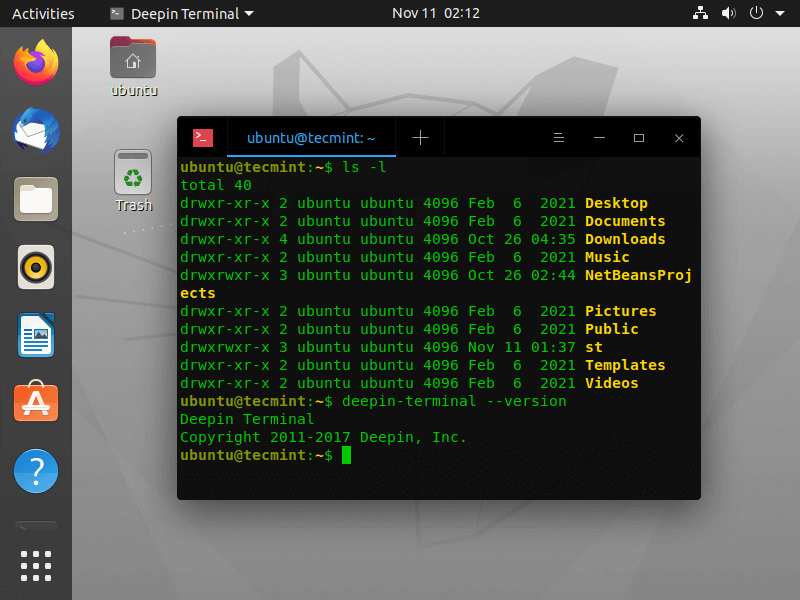
\includegraphics[width=\linewidth]{images/terminal.png}
        \end{center}
    \end{column}
\end{columns}

\pause

\begin{alertblock}{Engineering Perspective}
The terminal does not replace every graphical tool. Engineers select the most
appropriate interface: visual tools for observation and text commands for
repeatable, inspectable, and automatable workflows.
\end{alertblock}
\end{frame}





\begin{frame}{Terminal vs. Shell vs. Bash}
\framesubtitle{Untangling the command-line vocabulary}

\footnotesize

\begin{columns}[T]

    % --- LEFT: The Terminal ---
    \begin{column}{0.31\textwidth}
        \begin{block}{1. The Terminal}
            \textbf{The Window (The Phone)}
            \begin{itemize}
                \setlength{\itemsep}{0.2em}
                \item The graphical black box on your screen.
                \item It has no brain. It only captures your keyboard typing and displays text back to you.
            \end{itemize}
        \end{block}
    \end{column}

    % --- CENTER: The Shell ---
    \begin{column}{0.31\textwidth}
        \begin{block}{2. The Shell}
            \textbf{The Job Category (Translator)}
            \begin{itemize}
                \setlength{\itemsep}{0.2em}
                \item A type of software that acts as a middleman.
                \item It reads the text from the terminal and translates it into instructions the Operating System understands.
            \end{itemize}
        \end{block}
    \end{column}

    % --- RIGHT: Bash ---
    \begin{column}{0.34\textwidth}
        \begin{exampleblock}{3. Bash}
            \textbf{The Specific Brand}
            \begin{itemize}
                \setlength{\itemsep}{0.2em}
                \item \textbf{B}ourne \textbf{A}gain \textbf{SH}ell.
                \item The default shell installed on Ubuntu. 
                \item Other popular shells include \textbf{Zsh} (default on macOS) and \textbf{Fish}.
            \end{itemize}
        \end{exampleblock}
    \end{column}

\end{columns}

\pause
\vspace{0.3cm}

% --- BOTTOM: The Takeaway ---
\begin{alertblock}{The Information Flow}
    You type into the \textbf{Terminal} $\rightarrow$ The Terminal hands the text to \textbf{Bash} $\rightarrow$ \textbf{Bash} realizes \texttt{cd} means "Change Directory" and asks the \textbf{Kernel} to move you.
\end{alertblock}

\end{frame}


% -----------------------------------------------------------------------------
\begin{frame}{How to Read a Command}
\framesubtitle{A command normally combines a program, options, and arguments}

\footnotesize

\begin{center}
\colorbox{black!6}{
    \parbox[c][1.00cm][c]{0.88\textwidth}{
        \centering
        \ttfamily
        ls \quad -la \quad ~/quard\_um6p\_intership
    }
}
\end{center}

\vspace{0.15cm}

\begin{columns}[T,onlytextwidth]
    \begin{column}{0.31\textwidth}
        \begin{block}{Command}
            \texttt{ls}

            The program or shell command to execute.
        \end{block}
    \end{column}
    \begin{column}{0.31\textwidth}
        \begin{block}{Options}
            \texttt{-la}

            Modify behavior: long format and hidden files.
        \end{block}
    \end{column}
    \begin{column}{0.31\textwidth}
        \begin{block}{Argument}
            \texttt{~/quard\_um6p\_intership}

            The path on which the command operates.
        \end{block}
    \end{column}
\end{columns}

\pause

\begin{exampleblock}{General Pattern}
\centering
\texttt{command [options] [arguments]}
\end{exampleblock}

\begin{alertblock}{Important}
Spaces separate parts of a command. Paths containing spaces normally require
quotation marks or escaped spaces.
\end{alertblock}
\end{frame}

% -----------------------------------------------------------------------------
\begin{frame}{The Filesystem Is a Tree}
\framesubtitle{Every file and folder has a location called a path}

\footnotesize

\begin{columns}[T,onlytextwidth]
    \begin{column}{0.43\textwidth}
        \begin{block}{Important Locations}
            \begin{itemize}
                \setlength{\itemsep}{0.22em}
                \item \texttt{/}: root of the filesystem;
                \item \texttt{~}: current user's home directory;
                \item \texttt{.}: current directory;
                \item \texttt{..}: parent directory.
            \end{itemize}
        \end{block}
    \end{column}

    \begin{column}{0.53\textwidth}
        \begin{exampleblock}{Project Example}
            \texttt{~/quard\_um6p\_intership}

            \vspace{0.12cm}
            The tilde expands to the home directory. The remaining
            name identifies the internship repository inside that home directory.
        \end{exampleblock}
    \end{column}
\end{columns}

\pause

\begin{center}
\texttt{/home/student}
$\longrightarrow$
\texttt{quard\_um6p\_intership}
$\longrightarrow$
\texttt{gazebo}
$\longrightarrow$
\texttt{models}
\end{center}

\begin{alertblock}{Mental Model}
A path is a route through the filesystem tree. Navigation commands change the
current location; they do not move the project files themselves.
\end{alertblock}
\end{frame}

% -----------------------------------------------------------------------------
\begin{frame}[fragile]{Absolute and Relative Paths}
\framesubtitle{Two ways to describe the location of the same resource}

\footnotesize

\begin{columns}[T,onlytextwidth]
    \begin{column}{0.47\textwidth}
        \begin{block}{Absolute Path}
            Starts at the filesystem root \texttt{/} and describes the complete route.

\begin{verbatim}
/home/student/quard_um6p_intership/docs
\end{verbatim}

            It does not depend on the current directory.
        \end{block}
    \end{column}

    \begin{column}{0.47\textwidth}
        \begin{exampleblock}{Relative Path}
            Starts from the current directory.

\begin{verbatim}
docs
./docs
../another_folder
\end{verbatim}

            Its meaning depends on where the shell currently is.
        \end{exampleblock}
    \end{column}
\end{columns}

\begin{alertblock}{Common Mistake}
If a command reports ``No such file or directory,'' first run \texttt{pwd},
inspect the spelling and capitalization, and verify the path with \texttt{ls}.
Linux paths are case-sensitive.
\end{alertblock}
\end{frame}

% -----------------------------------------------------------------------------
\begin{frame}[fragile]{Locate Yourself and Inspect a Directory}
\framesubtitle{Begin every workflow by confirming context}

\footnotesize

\begin{block}{Purpose and Syntax}
\begin{verbatim}
pwd                 # print the current directory
ls [options] [path] # list directory contents
\end{verbatim}
\end{block}

\begin{columns}[T,onlytextwidth]
    \begin{column}{0.47\textwidth}
        \begin{exampleblock}{Simple Examples}
\begin{verbatim}
pwd
ls
ls -la
ls ~/Downloads
\end{verbatim}
        \end{exampleblock}
    \end{column}

    \begin{column}{0.47\textwidth}
        \begin{exampleblock}{Project Examples}
\begin{verbatim}
pwd
ls -la ~/quard_um6p_intership
ls gazebo/models
\end{verbatim}
        \end{exampleblock}
    \end{column}
\end{columns}

\begin{alertblock}{Common Mistakes}
Do not assume that a new terminal opens in the project directory. Hidden files
such as \texttt{.git} appear only when an option such as \texttt{-a} is used.
\end{alertblock}
\end{frame}

% -----------------------------------------------------------------------------
\begin{frame}[fragile]{Navigate with \texttt{cd}}
\framesubtitle{Change the shell's current working directory}

\footnotesize

\begin{block}{Purpose and Syntax}
\begin{verbatim}
cd [path]
\end{verbatim}
Without an argument, \texttt{cd} returns to the home directory.
\end{block}

\begin{columns}[T,onlytextwidth]
    \begin{column}{0.47\textwidth}
        \begin{exampleblock}{Navigation Examples}
\begin{verbatim}
cd ~
cd ..
cd -
cd ~/Documents
\end{verbatim}
        \end{exampleblock}
    \end{column}

    \begin{column}{0.47\textwidth}
        \begin{exampleblock}{Project Workflow}
\begin{verbatim}
cd ~/quard_um6p_intership
pwd
ls
cd gazebo/models
\end{verbatim}
        \end{exampleblock}
    \end{column}
\end{columns}

\begin{alertblock}{Common Mistakes}
\texttt{cd} requires a directory, not a regular file. Use tab completion to
avoid spelling errors, and run \texttt{pwd} whenever the current location is uncertain.
\end{alertblock}
\end{frame}

% -----------------------------------------------------------------------------
\begin{frame}[fragile]{Create Files and Directories}
\framesubtitle{Build a safe practice workspace before modifying the repository}

\footnotesize

\begin{block}{Purpose and Syntax}
\begin{verbatim}
mkdir [options] directory   # create a directory
touch file                  # create an empty file or update its time
\end{verbatim}
\end{block}

\begin{columns}[T,onlytextwidth]
    \begin{column}{0.47\textwidth}
        \begin{exampleblock}{Simple Examples}
\begin{verbatim}
mkdir bash_practice
touch notes.txt
mkdir -p logs/session_01
\end{verbatim}
        \end{exampleblock}
    \end{column}

    \begin{column}{0.47\textwidth}
        \begin{exampleblock}{Project Exercise}
\begin{verbatim}
cd ~/quard_um6p_intership
mkdir -p student_work/logs
touch student_work/observations.txt
\end{verbatim}
        \end{exampleblock}
    \end{column}
\end{columns}

\begin{alertblock}{Common Mistakes}
Without \texttt{-p}, \texttt{mkdir} cannot create missing parent directories.
Do not create random files inside source or configuration folders before
understanding their purpose.
\end{alertblock}
\end{frame}

% -----------------------------------------------------------------------------
\begin{frame}[fragile]{Copy and Move Safely}
\framesubtitle{Preserve originals before reorganizing or editing important files}

\footnotesize

\begin{block}{Purpose and Syntax}
\begin{verbatim}
cp [options] source destination
mv source destination
\end{verbatim}
\texttt{cp} duplicates data. \texttt{mv} relocates or renames it.
\end{block}

\begin{columns}[T,onlytextwidth]
    \begin{column}{0.47\textwidth}
        \begin{exampleblock}{Simple Examples}
\begin{verbatim}
cp notes.txt notes_backup.txt
cp -r config config_backup
mv notes.txt terminal_notes.txt
\end{verbatim}
        \end{exampleblock}
    \end{column}

    \begin{column}{0.47\textwidth}
        \begin{exampleblock}{Project Examples}
\begin{verbatim}
cp config/project.env \
   student_work/project.env.backup
mv student_work/observations.txt \
   student_work/day1_notes.txt
\end{verbatim}
        \end{exampleblock}
    \end{column}
\end{columns}

\vspace{-0.51cm}
\begin{alertblock}{Safety Check}
A destination file may be overwritten. Inspect both locations first, use clear
backup names, and remember that copying a directory normally requires \texttt{-r}.
\end{alertblock}
\end{frame}

% -----------------------------------------------------------------------------
\begin{frame}[fragile]{Remove Files with Care}
\framesubtitle{Deletion from the terminal may bypass the graphical trash folder}

\footnotesize

\begin{block}{Purpose and Syntax}
\begin{verbatim}
rm [options] file
rm -r directory
\end{verbatim}
\end{block}

\begin{exampleblock}{Safe Practice Example}
\begin{verbatim}
mkdir ~/bash_practice_remove
cd ~/bash_practice_remove
touch temporary.txt
ls
rm temporary.txt
ls
\end{verbatim}
\end{exampleblock}
\end{frame}


\begin {frame}[fragile]{Remove Files with Care}

\begin{alertblock}{High-Risk Command}
\texttt{rm} does not provide a general undo operation. Before deletion:
\begin{enumerate}
    \setlength{\itemsep}{0.15em}
    \item run \texttt{pwd};
    \item inspect the target with \texttt{ls};
    \item verify the exact path;
    \item avoid recursive or forced deletion unless it is truly necessary.
\end{enumerate}
Never copy and execute an unfamiliar deletion command from the internet.
\end{alertblock}

\end{frame}

% -----------------------------------------------------------------------------
\begin{frame}[fragile]{Read Text Files}
\framesubtitle{Select the viewer according to the amount of information}

\scriptsize

\begin{columns}[T,onlytextwidth]
    \begin{column}{0.48\textwidth}
        \begin{block}{Commands and Purposes}
\begin{verbatim}
cat file       # print the complete file
less file      # inspect interactively
head file      # show the first lines
tail file      # show the last lines
tail -f file   # follow appended output
\end{verbatim}
        \end{block}
    \end{column}

    \begin{column}{0.48\textwidth}
        \begin{exampleblock}{Project Examples}
\begin{verbatim}
cat README.md
less PHASE_3_PIPELINE_README.md
head -n 20 config/project.env
tail -n 30 student_work/run.log
tail -f student_work/run.log
\end{verbatim}
        \end{exampleblock}
    \end{column}
\end{columns}

\begin{block}{Practical Choice}
Use \texttt{cat} for short files, \texttt{less} for long documents,
\texttt{head} for introductions, and \texttt{tail} for recent logs.
Press \texttt{q} to leave \texttt{less} or stop \texttt{tail -f} with
\texttt{Ctrl+C}.
\end{block}

\begin{alertblock}{Common Mistake}
Printing a very large log with \texttt{cat} may hide the useful information in
thousands of terminal lines. Choose the smallest view that answers the question.
\end{alertblock}
\end{frame}

% -----------------------------------------------------------------------------
\begin{frame}[fragile]{Produce Output and Keep a Record}
\framesubtitle{Use \texttt{echo} and redirection to create simple evidence}

\footnotesize

\begin{block}{Purpose and Syntax}
\begin{verbatim}
echo "text"          # display text
command > file       # replace file content with output
command >> file      # append output to the file
\end{verbatim}
\end{block}

\begin{exampleblock}{Project Evidence Example}
\begin{verbatim}
echo "Day 1 terminal verification" > student_work/run.log
pwd >> student_work/run.log
ls -la >> student_work/run.log
echo "Inspection complete" >> student_work/run.log
cat student_work/run.log
\end{verbatim}
\end{exampleblock}
\end{frame}

% -----------------------------------------------------------------------------
\begin{frame}[fragile]{Find Files and Search Their Content}
\framesubtitle{Locate the resource first, then inspect the information inside it}

\scriptsize

\begin{block}{Purpose and Syntax}
\begin{verbatim}
find [start_path] [tests]           # search filesystem entries
grep [options] pattern [file]       # search text content
\end{verbatim}
\end{block}

\begin{columns}[T,onlytextwidth]
    \begin{column}{0.48\textwidth}
        \begin{exampleblock}{Simple Examples}
\begin{verbatim}
find . -name "*.py"
grep "camera" README.md
grep -n "error" student_work/run.log
\end{verbatim}
        \end{exampleblock}
    \end{column}

    \begin{column}{0.48\textwidth}
        \begin{exampleblock}{Project Examples}
\begin{verbatim}
find . -name "package.xml"
find gazebo/models -name "model.sdf"
grep -Rni "camera" docs
\end{verbatim}
        \end{exampleblock}
    \end{column}
\end{columns}

\begin{alertblock}{Common Mistakes}
Quote wildcard patterns such as \texttt{"*.py"} so the shell does not expand
them too early. Recursive searches can produce large outputs; begin from the
smallest relevant directory.
\end{alertblock}
\end{frame}

% % -----------------------------------------------------------------------------
% \begin{frame}[fragile]{Build a Pipeline with \texttt{|}}
% \framesubtitle{Send the output of one command into the input of another}

% \footnotesize

% \begin{center}
% \colorbox{black!6}{
%     \parbox[c][0.90cm][c]{0.88\textwidth}{
%         \centering
%         \ttfamily
%         producer \quad | \quad filter
%     }
% }
% \end{center}

% \begin{block}{Intuition}
% A pipe connects commands like software components in a robotics pipeline. The
% first command produces text; the next command filters or transforms that text.
% \end{block}

% \begin{exampleblock}{Examples}
% \begin{verbatim}
% ls -la | less
% history | grep "ros2"
% ps aux | grep "gz"
% find . -name "*.py" | sort
% \end{verbatim}
% \end{exampleblock}

% \begin{alertblock}{Interpretation Warning}
% \texttt{grep} may also display its own search process. A matching line proves
% that text was found; it does not automatically prove that the identified
% process or component is healthy.
% \end{alertblock}
% \end{frame}

% -----------------------------------------------------------------------------
\begin{frame}[fragile]{Chain Steps with \texttt{\&\&}}
\framesubtitle{Execute the next command only if the previous one succeeds}

\footnotesize

\begin{block}{Syntax and Meaning}
\begin{verbatim}
command_1 && command_2 && command_3
\end{verbatim}
Bash runs the chain from left to right and stops when one command returns a
failure status.
\end{block}

\begin{exampleblock}{Project Example}
\begin{verbatim}
cd ~/quard_um6p_intership && \
source config/project.env && \
pwd && \
ls gazebo/models
\end{verbatim}
\end{exampleblock}

\begin{alertblock}{Why This Is Safer Than Unconditional Execution}
If changing directory fails, the later commands are not executed in an
unexpected location. However, \texttt{\&\&} does not make a destructive command
safe; every command in the chain must still be reviewed.
\end{alertblock}
\end{frame}

% -----------------------------------------------------------------------------
\begin{frame}[fragile]{Environment Variables}
\framesubtitle{Named values used to configure processes and tools}

\footnotesize

\begin{block}{Intuition}
An environment variable is a named configuration value inherited by programs
started from the shell. It can describe paths, selected middleware, a world
name, or another runtime setting.
\end{block}

\begin{columns}[T,onlytextwidth]
    \begin{column}{0.47\textwidth}
        \begin{exampleblock}{Create and Read}
\begin{verbatim}
export WORLD_NAME="default"
echo "$WORLD_NAME"
\end{verbatim}
            \texttt{export} makes the variable available to child processes.
        \end{exampleblock}
    \end{column}

    \begin{column}{0.47\textwidth}
        \begin{exampleblock}{Project Configuration}
\begin{verbatim}
export GZ_SIM_RESOURCE_PATH="$HOME/.gz/models"
echo "$GZ_SIM_RESOURCE_PATH"
\end{verbatim}
        \end{exampleblock}
    \end{column}
\end{columns}

\begin{alertblock}{Common Mistakes}
Do not place spaces around \texttt{=}. Quote values containing spaces. Use
\texttt{\$NAME} to read a variable, and verify the value before launching a
process that depends on it.
\end{alertblock}
\end{frame}



\begin{frame}[fragile]{Why We Use \texttt{source}}
\framesubtitle{Apply configuration to the current shell session}

\footnotesize

\begin{columns}[T,onlytextwidth]

    % ---------------- LEFT COLUMN: Theory & Importance ---------------- %
    \begin{column}{0.48\textwidth}
        \begin{block}{Purpose and Syntax}
            \texttt{source} reads and executes a file \textbf{inside the current shell} rather than starting an isolated child shell. 
            
            \vspace{0.15cm}
            \textbf{Syntax:} \\
            \texttt{source filename} \\
            \texttt{.\ filename}
        \end{block}
        
        \begin{alertblock}{Why This Matters}
            Setup files modify environment variables. If you forget to source a file, your terminal remains "blind"---ROS 2 packages, executables, or Gazebo resources will not be discoverable.
            
            \vspace{0.15cm}
            \textit{Security Note:} Source only files you trust.
        \end{alertblock}
    \end{column}

    % ---------------- RIGHT COLUMN: Project Sequence ---------------- %
    \begin{column}{0.48\textwidth}
        \begin{exampleblock}{Typical Project Sequence}
            Every time you open a new terminal, you must "wake up" the robotics tools:
            
\begin{verbatim}
# 1. Load base ROS 2 tools
source /opt/ros/humble/setup.bash

# 2. Navigate to your workspace
cd ~/quard_um6p_intership

# 3. Load drone-specific variables
source config/project.env

# 4. Load your compiled code
source install/setup.bash
\end{verbatim}
        \end{exampleblock}
    \end{column}

\end{columns}

\end{frame}


% -----------------------------------------------------------------------------
\begin{frame}[fragile]{Comments and Readable Command Sequences}
\framesubtitle{A command should explain its intention as well as its action}

\footnotesize

\begin{block}{Comments with \texttt{\#}}
In Bash, text following \texttt{\#} is normally treated as a comment and is not
executed. Comments record purpose, assumptions, and expected observations.
\end{block}

\begin{exampleblock}{Project-Oriented Example}
\begin{verbatim}
# Load ROS 2 commands into this terminal
source /opt/ros/humble/setup.bash

# Enter the internship repository
cd ~/quard_um6p_intership

# Verify the selected Gazebo world
export WORLD_NAME="default"
echo "$WORLD_NAME"
\end{verbatim}
\end{exampleblock}

\end{frame}

% -----------------------------------------------------------------------------
\begin{frame}[fragile]{Permissions and \texttt{chmod}}
\framesubtitle{Control who may read, modify, or execute a file}

\footnotesize

\begin{block}{Read, Write, and Execute}
\begin{itemize}
    \setlength{\itemsep}{0.18em}
    \item \texttt{r}: read the content;
    \item \texttt{w}: modify the content;
    \item \texttt{x}: execute the file as a program or script.
\end{itemize}
\end{block}

\begin{columns}[T,onlytextwidth]
    \begin{column}{0.47\textwidth}
        \begin{exampleblock}{Inspect and Modify}
\begin{verbatim}
ls -l launch_project.sh
chmod +x launch_project.sh
ls -l launch_project.sh
\end{verbatim}
        \end{exampleblock}
    \end{column}

    \begin{column}{0.47\textwidth}
        \begin{exampleblock}{Execute Explicitly}
\begin{verbatim}
./launch_project.sh
\end{verbatim}
            The \texttt{./} path tells Bash to use the script in the current directory.
        \end{exampleblock}
    \end{column}
\end{columns}

\begin{alertblock}{Safety Concern}
Executable permission does not make a script trustworthy. Read unfamiliar
scripts before executing them, especially if they request elevated privileges.
\end{alertblock}
\end{frame}

% -----------------------------------------------------------------------------
\begin{frame}[fragile]{Administrative Commands and \texttt{sudo}}
\framesubtitle{Elevated privileges should be temporary, explicit, and justified}

\footnotesize

\begin{block}{What \texttt{sudo} Means}
\texttt{sudo command} runs one authorized command with elevated privileges.
It is used when a normal user is not permitted to change a protected system resource.
\end{block}

\begin{exampleblock}{Reasonable Use}
\begin{verbatim}
sudo apt update
sudo apt install package_name
\end{verbatim}
The password prompt may not display characters while typing. This is normal.
\end{exampleblock}

\begin{alertblock}{Safe Use Rules}
\begin{itemize}
    \setlength{\itemsep}{0.18em}
    % \item understand the complete command before executing it;
    \item verify the package name and installation source;
    \item do not add \texttt{sudo} merely to silence a permission error;
    \item avoid running project scripts as root unless documentation gives a valid reason;
    \item never execute an unknown internet command with elevated privileges.
\end{itemize}
\end{alertblock}
\end{frame}

% -----------------------------------------------------------------------------
\begin{frame}[fragile]{Install Software Safely with APT}
\framesubtitle{Use Ubuntu's package manager and verify each installation}

\footnotesize

\begin{block}{Two Different Operations}
\begin{verbatim}
sudo apt update
sudo apt install package_name
\end{verbatim}
\texttt{apt update} refreshes the package index. It does not upgrade every
installed package. \texttt{apt install} installs the requested package and dependencies.
\end{block}
\end{frame}


\begin{frame}[fragile]{Installing Software Packages}
\framesubtitle{Using the Advanced Packaging Tool (APT)}

\footnotesize

\begin{columns}[T,onlytextwidth]

    % ---------------- LEFT COLUMN: The Workflow ---------------- %
    \begin{column}{0.48\textwidth}
        \begin{exampleblock}{Safe Installation Workflow}
\begin{verbatim}
# 1. Update the list of available software
sudo apt update

# 2. Find the exact package name
apt search package_name

# 3. Install the package
sudo apt install package_name

# 4. Verify it was installed correctly
which installed_command
installed_command --help
\end{verbatim}
        \end{exampleblock}
    \end{column}

    % ---------------- RIGHT COLUMN: The Rules ---------------- %
    \begin{column}{0.48\textwidth}
        \begin{alertblock}{Project Rule: No Guessing}
            \begin{itemize}
                \setlength{\itemsep}{0.4em}
                \item \textbf{Trust the Docs:} Install only dependencies explicitly required by trusted project documentation.
                \item \textbf{Document Everything:} Record the exact package names and commands in your logbook so your teammates can reproduce the environment.
                \item \textbf{Stay Consistent:} Do not guess package names or mix unrelated installation methods (like \texttt{apt} vs. \texttt{pip} vs. \texttt{snap}) without understanding them.
            \end{itemize}
        \end{alertblock}
    \end{column}

\end{columns}

\end{frame}


% -----------------------------------------------------------------------------
\begin{frame}[fragile]{Programs and Processes}
\framesubtitle{A program is stored code; a process is a running instance}

\footnotesize

\begin{columns}[T,onlytextwidth]
    \begin{column}{0.42\textwidth}
        \begin{block}{Program}
            A file containing instructions, such as a Python script, ROS 2
            executable, or Gazebo binary.
        \end{block}
    \end{column}

    \begin{column}{0.54\textwidth}
        \begin{exampleblock}{Process}
            A running instance with a process identifier, memory, open files,
            environment variables, and operating state.
        \end{exampleblock}
    \end{column}
\end{columns}

\begin{block}{Inspect Running Processes}
\begin{verbatim}
ps
ps aux
ps aux | grep "gz"
ps aux | grep "python"
\end{verbatim}
\end{block}

\begin{alertblock}{Project Connection}
Gazebo, PX4, ROS 2 nodes, bridges, and AI programs run as separate processes.
A visible window is not the only evidence that a process exists, and an existing
process is not automatically a healthy process.
\end{alertblock}
\end{frame}

% -----------------------------------------------------------------------------
\begin{frame}[fragile]{Stop a Process Deliberately}
\framesubtitle{Prefer graceful interruption before sending stronger signals}

\footnotesize

\begin{block}{Normal Interactive Stop}
Press \texttt{Ctrl+C} in the terminal running the foreground process. This sends
an interrupt request and often allows the program to shut down cleanly.
\end{block}

\begin{exampleblock}{Stop by Process Identifier}
\begin{verbatim}
ps aux | grep "process_name"
kill PID
\end{verbatim}
First identify the correct process. Replace \texttt{PID} with its numeric identifier.
\end{exampleblock}

\begin{alertblock}{Safety and Diagnosis}
Do not kill processes by guesswork. Confirm the process owner and command first.
A forced stop can lose data or hide the original fault. Use stronger termination
only when graceful methods fail and the consequences are understood.
\end{alertblock}
\end{frame}

% -----------------------------------------------------------------------------
\begin{frame}[fragile]{Discover Commands and Documentation}
\framesubtitle{Ask the system before searching for random solutions}

\scriptsize

\begin{columns}[T,onlytextwidth]
    \begin{column}{0.48\textwidth}
        \begin{block}{Locate a Command}
\begin{verbatim}
which python3
which ros2
which gz
\end{verbatim}
\texttt{which} shows the executable selected through the shell's search path.
        \end{block}
    \end{column}

    \begin{column}{0.48\textwidth}
        \begin{exampleblock}{Read Usage Information}
\begin{verbatim}
ls --help
find --help
man ls
man chmod
\end{verbatim}
Press \texttt{q} to leave a manual page.
        \end{exampleblock}
    \end{column}
\end{columns}

\begin{alertblock}{Interpretation}
\texttt{--help} usually provides concise command-specific usage. \texttt{man}
provides structured reference documentation. \texttt{which} answers which
executable would run, not whether that program is correctly configured.
\end{alertblock}
\end{frame}

% -----------------------------------------------------------------------------
\begin{frame}{Terminal Productivity Habits}
\framesubtitle{Work faster without sacrificing accuracy}

\footnotesize

\begin{columns}[T,onlytextwidth]
    \begin{column}{0.48\textwidth}
        \begin{block}{Completion and History}
            \begin{itemize}
                \setlength{\itemsep}{0.22em}
                \item \textbf{Tab:} complete a path or command;
                \item \textbf{Up/Down:} browse previous commands;
                \item \textbf{Ctrl+R:} search command history;
                \item \texttt{history}: display numbered history;
                \item \texttt{clear}: clear the visible terminal.
            \end{itemize}
        \end{block}
    \end{column}

    \begin{column}{0.48\textwidth}
        \begin{exampleblock}{Editing and Control}
            \begin{itemize}
                \setlength{\itemsep}{0.22em}
                \item \textbf{Ctrl+C:} interrupt the current process;
                \item \textbf{Ctrl+L:} clear the screen;
                \item \textbf{Ctrl+A:} move to line start;
                \item \textbf{Ctrl+E:} move to line end;
                \item \textbf{Ctrl+U:} erase to line start.
            \end{itemize}
        \end{exampleblock}
    \end{column}
\end{columns}

\begin{alertblock}{Safety Habit}
History saves time, but never re-run a recalled command automatically. Read the
entire line and verify paths, variables, and options before pressing Enter.
\end{alertblock}
\end{frame}

% -----------------------------------------------------------------------------
\begin{frame}[fragile]{Read Error Messages as Evidence}
% \framesubtitle{The first useful response to failure is observation, not random modification}

\footnotesize

\begin{block}{A Disciplined Diagnostic Sequence}
\begin{enumerate}
    \setlength{\itemsep}{0.18em}
    \item identify the command that failed;
    \item read the first meaningful error and its context;
    \item classify the problem: path, permission, command, dependency, syntax, or process;
    % \item inspect the relevant state with a small verification command;
    \item change one factor and execute again.
\end{enumerate}
\end{block}

\begin{exampleblock}{Typical Messages and First Checks}
\begin{verbatim}
command not found            -> which command; check setup
No such file or directory    -> pwd; ls; inspect spelling
Permission denied            -> ls -l; inspect ownership and mode
package not found            -> apt update; verify package name
\end{verbatim}
\end{exampleblock}

\begin{alertblock}{Do Not Hide the Problem}
Adding \texttt{sudo}, reinstalling everything, or killing every process may
change the symptom without identifying the cause. Preserve the original command
and output before troubleshooting.
\end{alertblock}
\end{frame}

% -----------------------------------------------------------------------------
\begin{frame}{Common Command-Line Mistakes}
\framesubtitle{Small syntax errors can change the meaning of an operation}

\scriptsize

\begin{columns}[T,onlytextwidth]
    \begin{column}{0.48\textwidth}
        \begin{block}{Context and Paths}
            \begin{itemize}
                \setlength{\itemsep}{0.18em}
                \item running a command from the wrong directory;
                \item confusing absolute and relative paths;
                \item ignoring capitalization;
                \item forgetting quotation marks around spaces;
                \item assuming \texttt{~} means the project root.
            \end{itemize}
        \end{block}
    \end{column}

    \begin{column}{0.48\textwidth}
        \begin{block}{Syntax and System State}
            \begin{itemize}
                \setlength{\itemsep}{0.18em}
                \item inserting spaces around variable assignment;
                \item forgetting to source a setup file;
                \item confusing \texttt{>} with \texttt{>>};
                \item using \texttt{sudo} as a universal repair;
                \item copying commands without reading their outputs.
            \end{itemize}
        \end{block}
    \end{column}
\end{columns}

\begin{alertblock}{Reliable Recovery}
Return to known facts: \texttt{pwd}, \texttt{ls -la}, \texttt{echo "\$VARIABLE"},
\texttt{which command}, \texttt{ps aux}, and the complete error message.
\end{alertblock}
\end{frame}









% ----------------------------------------------------------------------------
% MINI-PROJECT FRAME 1: Initialization
% ----------------------------------------------------------------------------
\begin{frame}[fragile]{Terminal Sandbox (Part 1/3)}
\framesubtitle{Environment Initialization and Navigation}

\footnotesize

\begin{columns}[T,onlytextwidth]

    % --- LEFT COLUMN: The Mission ---
    \begin{column}{0.48\textwidth}
        \begin{block}{1. Access the Sandbox}
            Open your browser to the free online terminal:
            \vspace{0.1cm} \\
            \textbf{\href{https://webterm.app/en/free-play}{\color{um6p-color-dark-blue}webterm.app/en/free-play}}
        \end{block}

        \begin{exampleblock}{Mission 1: The Workspace}
            Before writing code, an engineer must orient themselves and build a clean folder structure.
            \begin{enumerate}
                \setlength{\itemsep}{0.2em}
                \item Print your current working directory.
                \item List the existing files.
                \item Create a new folder named \texttt{drone\_ws}.
                \item Move inside \texttt{drone\_ws}.
                \item Verify that the folder is currently empty.
            \end{enumerate}
        \end{exampleblock}
    \end{column}

    \pause
    % --- RIGHT COLUMN: The Solution ---
    \begin{column}{0.48\textwidth}
        \begin{block}{Mission 1: Solution Workflow}
            \textit{Try to complete the mission first. Use this solution if you get stuck:}
            
\begin{verbatim}
# 1. Print Working Directory
pwd
# 2. List current files
ls -la
# 3. Create the workspace directory
mkdir drone_ws
# 4. Change directory into it
cd drone_ws
# 5. List files (should be empty)
ls
\end{verbatim}
        \end{block}
    \end{column}

\end{columns}
\end{frame}


% ----------------------------------------------------------------------------
% MINI-PROJECT FRAME 2: File Manipulation
% ----------------------------------------------------------------------------
\begin{frame}[fragile]{Terminal Sandbox (Part 2/3)}
\framesubtitle{Creating, Reading, and Copying Files}

\footnotesize

\begin{columns}[T,onlytextwidth]

    % --- LEFT COLUMN: The Mission ---
    \begin{column}{0.48\textwidth}
        \begin{exampleblock}{Mission 2: Configuration Files}
            A drone needs configuration parameters. Let's create a file, write data into it, and back it up.
            \begin{enumerate}
                \setlength{\itemsep}{0.2em}
                \item Use \texttt{echo} to create a file named \texttt{config.env} containing the text \texttt{ROS\_DOMAIN\_ID=42}.
                \item Read the contents of \texttt{config.env} directly in the terminal to verify.
                \item Create a new folder named \texttt{backup}.
                \item Copy \texttt{config.env} into the \texttt{backup} folder.
            \end{enumerate}
        \end{exampleblock}
    \end{column}

    \pause
    % --- RIGHT COLUMN: The Solution ---
    \begin{column}{0.48\textwidth}
        \begin{block}{Mission 2: Solution Workflow}
            
\begin{verbatim}
# 1. Write text into a new file
echo "ROS_DOMAIN_ID=42" > config.env
# 2. Read (concatenate) the file
cat config.env
# 3. Create a backup folder
mkdir backup
# 4. Copy the file into the folder
cp config.env backup/
# Verify the copy was successful
ls backup/
\end{verbatim}
        \end{block}
    \end{column}

\end{columns}
\end{frame}


% ----------------------------------------------------------------------------
% MINI-PROJECT FRAME 3: Advanced Operations
% ----------------------------------------------------------------------------
\begin{frame}[fragile]{Terminal Sandbox (Part 3/3)}
\framesubtitle{Moving, Searching, and Cleanup}

\footnotesize

\begin{columns}[T,onlytextwidth]

    % --- LEFT COLUMN: The Mission ---
    \begin{column}{0.48\textwidth}
        \begin{exampleblock}{Mission 3: System Administration}
            Engineers must regularly restructure projects and search through massive log files.
            \begin{enumerate}
                \setlength{\itemsep}{0.2em}
                \item Rename your \texttt{backup} folder to \texttt{archive}.
                \item Use the \texttt{grep} command to search for the word \texttt{ROS} inside your archived configuration file.
                \item Finally, clean up your workspace by permanently deleting the entire \texttt{archive} folder.
            \end{enumerate}
        \end{exampleblock}
        
        \begin{alertblock}{Danger Zone: \texttt{rm -rf}}
            In Linux, there is no "Recycle Bin" for the terminal. The \texttt{rm} command deletes files instantly and permanently. Use it with extreme caution!
        \end{alertblock}
    \end{column}

    \pause
    % --- RIGHT COLUMN: The Solution ---
    \begin{column}{0.48\textwidth}
        \begin{block}{Mission 3: Solution Workflow}
            
\begin{verbatim}
# 1. Rename (Move) backup to archive
mv backup archive
# Verify the name changed
ls
# 2. Search for "ROS" inside the file
grep "ROS" archive/config.env
# 3. Delete the archive folder 
# (-r = recursive, -f = force)
rm -rf archive/
# Verify it is gone forever
ls
\end{verbatim}
        \end{block}
    \end{column}

\end{columns}
\end{frame}



\begin{frame}{References and Further Reading}
\framesubtitle{Essential documentation for Day 1 foundations}

            \begin{thebibliography}{9}
                \bibitem{linuxcmd} William E. Shotts Jr.
                \newblock \emph{The Linux Command Line}.
                \newblock \href{https://linuxcommand.org/}{\color{um6p-color-dark-blue}linuxcommand.org}

                \bibitem{ubuntutut} Canonical Ltd.
                \newblock \emph{Ubuntu Command Line for Beginners}.
                \newblock \href{https://ubuntu.com/tutorials/command-line-for-beginners}{\color{um6p-color-dark-blue}ubuntu.com/tutorials}

                \bibitem{progit} Scott Chacon \& Ben Straub.
                \newblock \emph{Pro Git Book}.
                \newblock \href{https://git-scm.com/book/en/v2}{\color{um6p-color-dark-blue}git-scm.com/book}
            \end{thebibliography}
\end{frame}



\begin{frame}{Transition to the Technical Foundations}
\framesubtitle{One foundation completed, the next one begins}

% \footnotesize

% ------------------------------------------------------------------
% CURRENT PROGRESS
% ------------------------------------------------------------------
\begin{center}
    \textbf{\color{um6p-dark}Internship Learning Roadmap}
\end{center}

\vspace{0.15cm}

\begin{center}
\renewcommand{\arraystretch}{1.15}
\begin{tabular}{c@{\hspace{0.10cm}}c@{\hspace{0.10cm}}c@{\hspace{0.10cm}}c@{\hspace{0.10cm}}c}

% Completed foundation
\colorbox{um6p-color-dark-green!20}{
    \parbox[c][0.85cm][c]{1.65cm}{
        \centering
        \scriptsize\bfseries
        Ubuntu\\
        \textcolor{um6p-color-dark-green}{Completed}
    }
}


& $\longrightarrow$ &

% Completed foundation
\colorbox{um6p-color-dark-green!20}{
    \parbox[c][1.05cm][c]{2.15cm}{
        \centering
        \scriptsize\bfseries
        Terminal\\
        and Bash\\[-0.05cm]
        \textcolor{um6p-color-dark-green}{Completed}
    }
}

& $\longrightarrow$ &

% Upcoming foundations
\colorbox{um6p-color-light-blue}{
    \parbox[c][0.85cm][c]{1.65cm}{
        \centering
        \scriptsize
        Git and\\
        GitHub \\[-0.05cm]
        \textcolor{um6p-dark}{Current}
    }
}

\\[0.25cm]

\colorbox{black!7}{
    \parbox[c][0.85cm][c]{1.65cm}{
        \centering
        \scriptsize
        Python for\\
        Robotics
    }
}

& $\longrightarrow$ &

\colorbox{black!7}{
    \parbox[c][0.85cm][c]{2.15cm}{
        \centering
        \scriptsize
        ROS 2
    }
}

& $\longrightarrow$ &

\colorbox{black!7}{
    \parbox[c][0.85cm][c]{1.65cm}{
        \centering
        \scriptsize
        Gazebo\\
        and PX4
    }
}

\end{tabular}

\vspace{0.15cm}

\colorbox{black!7}{
    \parbox[c][0.75cm][c]{2.1cm}{
        \centering
        \scriptsize
        AI Integration
    }
}
\end{center}


\end{frame}
